\documentclass[11pt]{article}

\usepackage[margin=1in]{geometry}
\usepackage[T1]{fontenc}
\usepackage[utf8]{inputenc}
\usepackage{lmodern}
\usepackage{amsmath,amssymb}
\usepackage{graphicx}
\usepackage{booktabs}
\usepackage{hyperref}
\usepackage{natbib}
\usepackage{xcolor}
\usepackage{caption}
\usepackage{subcaption}
\usepackage{multirow}

\title{The Hop-Count Cliff: Characterizing the Breakdown of\\Graph Retrieval Strategies on Dense Knowledge Graphs}
\author{
  Matt Krasnow \and Seager Hunt \and Cory Wu \and Reade Park \\
  \textit{Stat 175: Networks} \\
  \textit{Harvard University}
}
\date{Spring 2026}

\begin{document}

\maketitle

\begin{abstract}
We investigate how retrieval strategy affects answer quality in graph retrieval-augmented generation (GraphRAG) as query complexity increases. Through a controlled experiment on the STaRK-PrimeKG benchmark (129K nodes, 4M edges, 11,204 queries), we compare four retrieval strategies---node-centric, path-centric, subgraph-centric, and hybrid---stratified by the number of relational hops required to reach the answer. We find a sharp \textit{performance cliff} from 1-hop to 2-hop queries across all strategies, rather than the gradual phase transition we hypothesized. Hit@10 drops approximately 70\% at this boundary. Logistic regression confirms a significant strategy$\times$hop-count interaction ($\beta = +2.09$), indicating structural methods gain relative advantage as complexity increases. Ablation studies reveal a fundamental focus-versus-coverage tradeoff: configurations that maximize 1-hop performance (e.g., single-seed subgraph expansion achieving Hit@10 $= 0.77$) completely fail at multi-hop, while broader configurations that help multi-hop dilute 1-hop accuracy. We argue this tradeoff, driven by the high density of real-world knowledge graphs, implies that effective GraphRAG requires query-adaptive retrieval rather than any fixed strategy.
\end{abstract}

%----------------------------------------------------------------------
\section{Introduction}
%----------------------------------------------------------------------

Retrieval-augmented generation (RAG) has become a standard approach for grounding large language model (LLM) outputs in external knowledge~\citep{lewis2020retrieval}. While traditional RAG retrieves text passages via vector similarity, \textit{graph} RAG (GraphRAG) leverages the relational structure of knowledge graphs (KGs) to retrieve more contextually relevant information. Recent work has proposed diverse retrieval strategies including subgraph extraction~\citep{hu2024grag}, path-based reasoning~\citep{yu2025graphflow}, and hybrid structural-textual mixtures~\citep{yue2025mor}.

A natural question arises: \textit{when does graph structure actually help?} All three approaches report improvements over text-only baselines, but none systematically varies query complexity to identify the boundary where structural retrieval becomes necessary. \citet{yue2025mor} report ``uneven retrieving performance across different query logics'' without characterizing the unevenness, and \citet{yu2025graphflow} critique retrieval fidelity without isolating hop count as a variable.

We address this gap with a controlled experiment that isolates query hop count---the number of relational hops from the query entity to the answer---as the independent variable. We hypothesized that a phase transition exists at some critical hop count $h^*$ where structural retrieval overtakes text-only retrieval. Our findings are more striking: rather than a gradual crossover, we observe a \textit{cliff}---a catastrophic drop in performance from 1-hop to 2-hop queries for \textit{all} strategies, followed by a low plateau. The phase transition exists not between strategies but between solvable and nearly unsolvable queries.

Our contributions are:
\begin{enumerate}
    \item We characterize the \textbf{hop-count cliff}: a sharp performance boundary at 2 hops on dense text-rich KGs where all retrieval strategies collapse.
    \item We provide statistical evidence (paired bootstrap tests, logistic regression interaction analysis) that structural methods \textbf{gain relative advantage} as query complexity increases, even though absolute performance is low.
    \item Through five ablation studies, we identify a \textbf{fundamental focus-vs-coverage tradeoff} that no single hyperparameter setting resolves, suggesting the need for query-adaptive retrieval.
\end{enumerate}

%----------------------------------------------------------------------
\section{Related Work}
%----------------------------------------------------------------------

\paragraph{Graph RAG.} \citet{hu2024grag} introduce GRAG, which retrieves subgraphs around query-relevant entities and encodes them via a graph neural network before passing to an LLM. They demonstrate improvements on commonsense reasoning (ExplaGraphs) and multi-hop QA (WebQSP) but do not analyze performance as a function of hop count.

\paragraph{Hybrid Retrieval.} \citet{yue2025mor} propose MoR (Mixture of Retrieval), which interweaves structural traversal and textual matching through a Planning-Reasoning-Organizing framework. They evaluate on STaRK~\citep{wu2024stark} and note uneven performance across query logics, motivating our systematic investigation of this unevenness.

\paragraph{Retrieval Fidelity.} \citet{yu2025graphflow} critically examine whether KG-based RAG actually retrieves what is needed, introducing GraphFlow, a flow-based retrieval method. They show existing methods often fail to retrieve relevant context but focus on proposing a solution rather than characterizing when and why failure occurs.

\paragraph{STaRK Benchmark.} \citet{wu2024stark} introduce STaRK, a benchmark for semi-structured retrieval over text-rich knowledge bases covering three domains (biomedical, e-commerce, academic). We use STaRK-PrimeKG as our primary evaluation setting, as it is used by both MoR and GraphFlow, enabling direct comparison.

%----------------------------------------------------------------------
\section{Experimental Design}
%----------------------------------------------------------------------

\subsection{Dataset}

We use STaRK-PrimeKG~\citep{wu2024stark}, a biomedical knowledge graph derived from PrimeKG~\citep{chandak2023primekg}. Table~\ref{tab:graph_stats} summarizes its properties.

\begin{table}[h]
\centering
\caption{STaRK-PrimeKG graph properties.}
\label{tab:graph_stats}
\begin{tabular}{lr}
\toprule
Property & Value \\
\midrule
Nodes & 129,375 \\
Edges & 4,049,642 \\
Mean degree & 62.6 \\
Median degree & 4.0 \\
Max degree & 17,355 \\
Clustering coefficient & 0.079 \\
Connected components & 1 \\
Approx.\ diameter & 15 \\
\bottomrule
\end{tabular}
\end{table}

The graph is dense (mean degree 62.6) with a highly skewed degree distribution (median 4.0 vs.\ mean 62.6), indicating the presence of high-degree hub nodes characteristic of biological networks.

\subsection{Hop-Count Stratification}

We stratify the 11,204 QA pairs by the shortest path length from the query entity to the gold answer in the knowledge graph. Since STaRK does not provide explicit query entity IDs, we identify the query entity as the graph node whose text embedding is most similar to the query (using all-MiniLM-L6-v2~\citep{reimers2019sentence}). We then compute the shortest path to each gold answer node via BFS.

\begin{table}[h]
\centering
\caption{Distribution of QA pairs by hop count.}
\label{tab:hop_dist}
\begin{tabular}{lrr}
\toprule
Hop Count & $n$ & \% of Total \\
\midrule
1-hop & 3,851 & 34.4\% \\
2-hop & 3,699 & 33.0\% \\
3-hop & 2,193 & 19.6\% \\
4-hop & 1,001 & 8.9\% \\
5-hop & 313 & 2.8\% \\
6+-hop & 147 & 1.3\% \\
\bottomrule
\end{tabular}
\end{table}

All bins contain $\geq 50$ samples, providing sufficient statistical power for pairwise tests.

\subsection{Retrieval Strategies}

We implement four retrieval strategies, each taking a natural language query and returning a ranked list of candidate node IDs:

\begin{enumerate}
    \item \textbf{Node-centric} (text-only baseline): Retrieve the top-$k$ nodes by cosine similarity between the query embedding and node text embeddings. This ignores graph structure entirely.

    \item \textbf{Path-centric} (inspired by GraphFlow~\citep{yu2025graphflow}): Identify seed nodes via embedding similarity, compute shortest paths between all seed pairs, score paths by average node-query similarity, and return nodes from the highest-scoring paths.

    \item \textbf{Subgraph-centric} (inspired by GRAG~\citep{hu2024grag}): Identify seed nodes, expand by $k$ hops, cap the subgraph size via relevance-based pruning, and return nodes ranked by embedding similarity within the subgraph.

    \item \textbf{Hybrid} (inspired by MoR~\citep{yue2025mor}): Combine textual similarity scores and structural proximity scores with a tunable weight parameter $\alpha \in [0, 1]$.
\end{enumerate}

\subsection{Controls}

All strategies use the same embedding model (all-MiniLM-L6-v2) and shared FAISS index. We evaluate retrieval quality directly via Hit@$k$ and MRR rather than end-to-end generation quality, isolating the retrieval component.

\subsection{Statistical Methods}

\begin{itemize}
    \item \textbf{Paired bootstrap tests} ($B = 10{,}000$) for pairwise strategy comparisons at each hop count.
    \item \textbf{Logistic regression} with features (hop count, is\_structural, hop $\times$ is\_structural) to test the interaction between strategy type and query complexity on Hit@1.
    \item \textbf{Cohen's $d$} effect sizes to quantify practical significance.
\end{itemize}

%----------------------------------------------------------------------
\section{Results}
%----------------------------------------------------------------------

\subsection{The Hop-Count Cliff}

Figure~\ref{fig:phase_transition} shows retrieval performance as a function of hop count for all four strategies. The dominant feature is a \textit{cliff}: Hit@10 drops approximately 70\% from 1-hop to 2-hop across all strategies, then plateaus at low values through 6+ hops.

\begin{figure}[h]
    \centering
    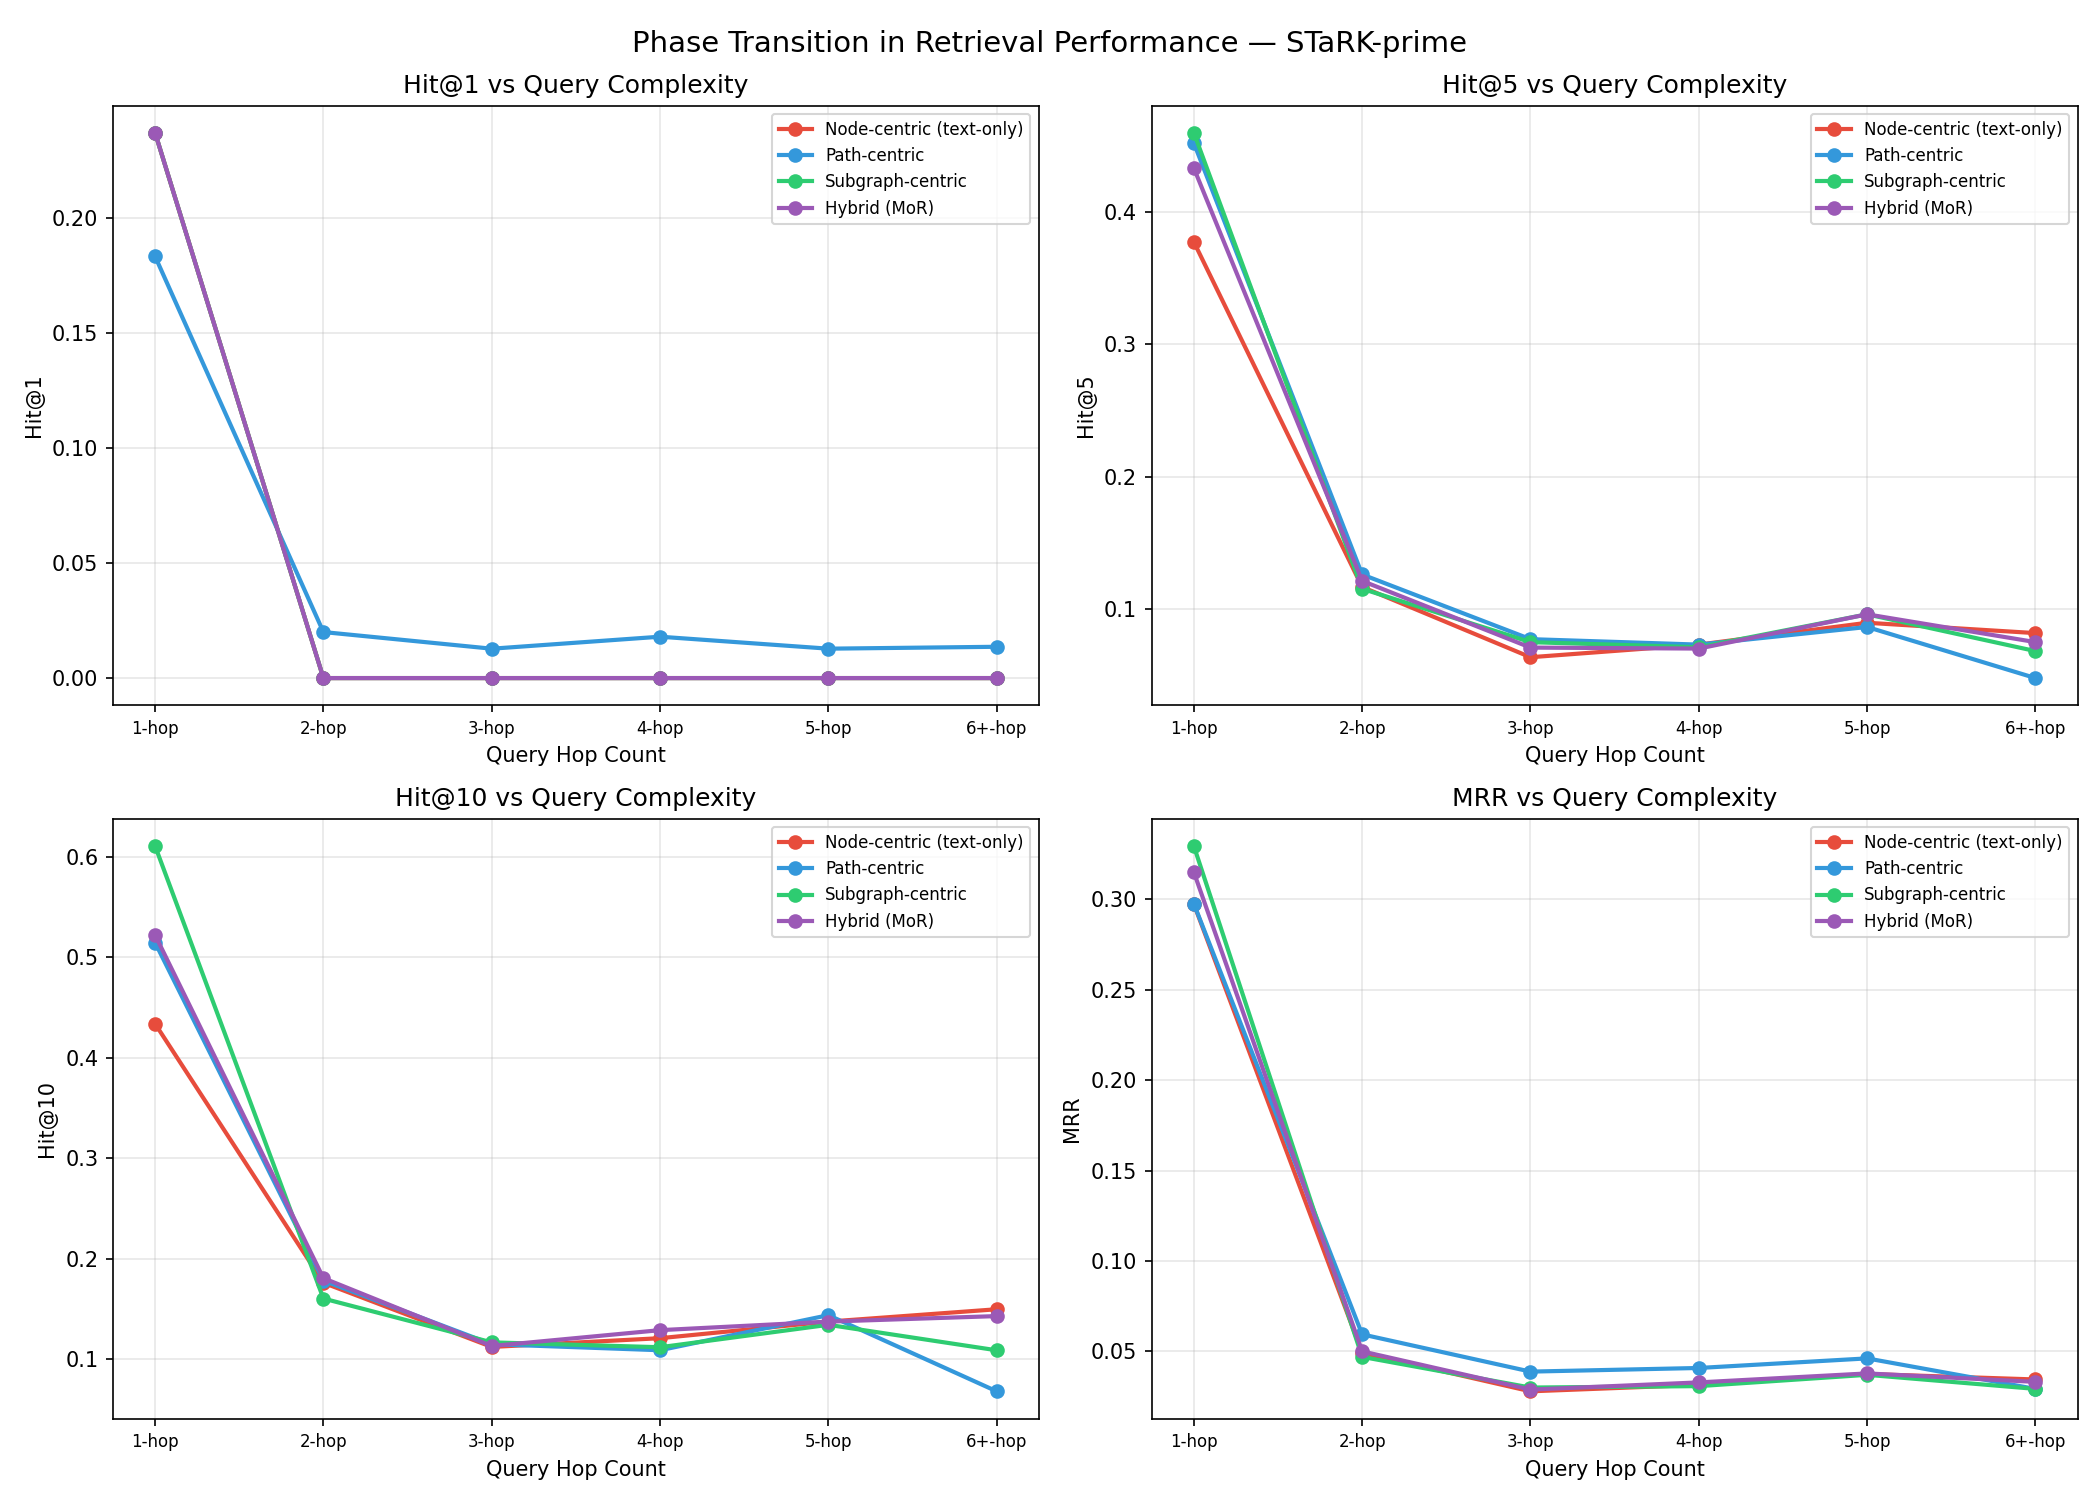
\includegraphics[width=\textwidth]{../results/prime_phase_transition.png}
    \caption{Retrieval performance vs.\ query hop count for all four strategies on STaRK-PrimeKG ($n = 11{,}204$). A sharp cliff appears between 1-hop and 2-hop queries.}
    \label{fig:phase_transition}
\end{figure}

Table~\ref{tab:main_results} presents the full results. At 1-hop, subgraph-centric retrieval achieves the highest Hit@10 (0.611), substantially outperforming the node-centric baseline (0.434). At 2+ hops, all strategies perform poorly, though path-centric is the only strategy with Hit@1 $> 0$.

\begin{table}[h]
\centering
\caption{Hit@10 and MRR by hop count and retrieval strategy. Bold indicates best per row.}
\label{tab:main_results}
\begin{tabular}{l cccc cccc}
\toprule
& \multicolumn{4}{c}{Hit@10} & \multicolumn{4}{c}{MRR} \\
\cmidrule(lr){2-5} \cmidrule(lr){6-9}
Hop & Node & Path & Subgraph & Hybrid & Node & Path & Subgraph & Hybrid \\
\midrule
1 & 0.434 & 0.514 & \textbf{0.611} & 0.522 & 0.297 & 0.297 & \textbf{0.329} & 0.315 \\
2 & 0.176 & 0.178 & 0.160 & \textbf{0.181} & 0.049 & \textbf{0.060} & 0.047 & 0.050 \\
3 & 0.112 & 0.115 & \textbf{0.117} & 0.113 & 0.028 & \textbf{0.039} & 0.030 & 0.029 \\
4 & 0.121 & 0.109 & 0.112 & \textbf{0.129} & 0.032 & \textbf{0.041} & 0.031 & 0.033 \\
5 & 0.137 & \textbf{0.144} & 0.134 & 0.137 & 0.038 & \textbf{0.046} & 0.037 & 0.038 \\
6+ & \textbf{0.150} & 0.068 & 0.109 & 0.143 & \textbf{0.035} & 0.029 & 0.029 & 0.033 \\
\bottomrule
\end{tabular}
\end{table}

\subsection{Statistical Analysis}

\paragraph{Interaction effect.} Logistic regression on Hit@1 with features (hop count, is\_structural, hop $\times$ structural) yields an interaction coefficient of $\beta = +2.09$, confirming that structural methods gain relative advantage as hop count increases.

\paragraph{Pairwise tests.} Paired bootstrap tests ($B = 10{,}000$) show that path-centric retrieval significantly outperforms node-centric on Hit@1 at 2-hop through 5-hop ($p < 0.05$, Cohen's $d = 0.16$--$0.20$). However, the absolute differences are small (1--2 percentage points). Subgraph-centric retrieval significantly outperforms node-centric on MRR at 1-hop ($p < 0.001$, $d = 0.08$).

\subsection{Ablation Studies}

We conduct five ablation studies on a subsample of 200 queries per hop-count bin to understand the sensitivity of each strategy to its key hyperparameters.

\paragraph{Ablation 1: Top-$k$ budget.} Increasing $k$ from 1 to 50 in node-centric retrieval improves Hit@$k$ (trivially) but MRR increases only from 0.30 to 0.36 at 1-hop. The answer's rank does not improve; wider retrieval simply casts a broader net.

\paragraph{Ablation 2: $k$-hop expansion depth.} For subgraph-centric retrieval, $k = 1$ achieves the best 1-hop performance (Hit@10 $= 0.64$). Expanding to $k = 2$ hops \textit{hurts} 1-hop performance (0.48) while providing only a modest gain at 2-hop (0.30 vs.\ 0.24). This is explained by the graph's high mean degree: a 2-hop expansion from 3 seed nodes potentially touches $\sim$3,600 nodes, flooding the subgraph with irrelevant context. Relevance-based pruning partially mitigates this but cannot overcome the signal-to-noise collapse.

\paragraph{Ablation 3: Path length.} Shorter paths ($\ell = 2$) yield higher MRR at 2-hop (0.107) compared to longer paths ($\ell = 5$, MRR $= 0.089$). In a dense graph where many paths exist between any two nodes, shorter, more direct connections carry more information.

\paragraph{Ablation 4: Number of seed nodes.} This ablation reveals the clearest tradeoff. With a single seed, subgraph-centric retrieval achieves its peak 1-hop performance (Hit@10 $= 0.77$, MRR $= 0.45$)---the highest in any experiment---but \textit{completely zeros out} at 2+ hops. Increasing to 10 seeds helps multi-hop (Hit@10 $= 0.26$ at 2-hop) but reduces 1-hop to 0.46. No single seed count works across complexity levels.

\paragraph{Ablation 5: Hybrid text weight.} The optimal mixture weight $\alpha$ shifts with query complexity: $\alpha = 0.2$ (mostly structural) is best for 1-hop (Hit@10 $= 0.57$), while $\alpha = 0.5$--$0.6$ (balanced) is best for multi-hop. Pure structural ($\alpha = 0.0$) performs worst overall, confirming that textual similarity provides essential signal even when graph structure is available.

%----------------------------------------------------------------------
\section{Discussion}
%----------------------------------------------------------------------

\subsection{Why the Cliff?}

The hop-count cliff is a consequence of graph density. On STaRK-PrimeKG, the mean degree is 62.6, meaning a single hop from a query entity reaches $\sim$60 nodes. At 1-hop, the answer is likely within this immediate neighborhood, and all structural methods can find it. At 2-hop, the answer is somewhere among $\sim$3,600 second-degree neighbors, and embedding similarity alone cannot reliably distinguish the correct answer from thousands of structurally similar alternatives.

This explains why the cliff is sharp rather than gradual: the combinatorial explosion of the neighborhood happens discretely at each hop, and there is no intermediate regime where partial structural information helps.

\subsection{The Focus-vs-Coverage Tradeoff}

Our ablations reveal that every hyperparameter controlling retrieval breadth (number of seeds, expansion depth, path length, text weight) exhibits the same pattern: settings that maximize 1-hop performance minimize multi-hop performance and vice versa. This is not a limitation of our specific implementations but a structural property of retrieval on dense graphs: \textit{the information needed to reach multi-hop answers is diffused across many graph paths, and any strategy that focuses enough to avoid noise at 1-hop will miss the signal at higher hops.}

\subsection{Connections to Prior Work}

Our results provide empirical grounding for observations in the literature:
\begin{itemize}
    \item \citet{yue2025mor}'s ``uneven performance across query logics'' is not merely uneven---it is a cliff, with fundamentally different regimes above and below 2 hops.
    \item \citet{yu2025graphflow}'s finding that GraphRAG ``doesn't always retrieve what you need'' is explained by the density-driven noise that overwhelms structural signal at higher hop counts.
    \item The success of \citet{yue2025mor}'s planning stage can be understood as an implicit mechanism for adapting retrieval breadth to estimated query complexity.
\end{itemize}

\subsection{Implications}

Our results suggest that effective GraphRAG on dense knowledge graphs requires \textbf{query-adaptive retrieval}: a system that estimates query complexity (e.g., the number of reasoning hops required) and adjusts its retrieval strategy accordingly. Fixed-strategy approaches will either excel at simple queries and fail at complex ones, or sacrifice simple-query performance for marginal multi-hop gains.

\subsection{Limitations}

Our retrievers are relatively simple implementations that serve as controlled baselines rather than state-of-the-art systems. The papers we build on use more sophisticated approaches (learned planners, GNN encoders, LLM-guided traversal). Our contribution is characterizing the hop-count cliff and the focus-vs-coverage tradeoff, not claiming that our implementations are optimal.

We evaluate on a single dataset (STaRK-PrimeKG). While the biomedical domain provides a dense, well-connected graph that clearly exhibits the phenomena we describe, generalization to sparser graphs or other domains remains to be tested.

Our hop-count stratification relies on identifying the query entity via embedding similarity, which introduces noise. Some queries may be assigned to incorrect hop-count bins, potentially smoothing the observed cliff.

%----------------------------------------------------------------------
\section{Conclusion}
%----------------------------------------------------------------------

We set out to find a phase transition in GraphRAG retrieval performance and found something more fundamental: a \textit{cliff}. On dense knowledge graphs, all retrieval strategies---text-only, path-based, subgraph-based, and hybrid---collapse at 2-hop queries, with no strategy able to reliably recover. The statistical evidence confirms that structural methods do gain relative advantage at higher hop counts, but the absolute performance is too low for practical use.

Through systematic ablation studies, we show that this cliff arises from a fundamental focus-versus-coverage tradeoff inherent to dense graphs. The implication is clear: the future of GraphRAG lies not in better fixed retrieval strategies but in systems that adapt their retrieval approach to the complexity of each query.

%----------------------------------------------------------------------
\bibliographystyle{plainnat}
\begin{thebibliography}{10}

\bibitem[Chandak et al.(2023)]{chandak2023primekg}
Chandak, P., Huang, K., and Zitnik, M.
\newblock Building a knowledge graph to enable precision medicine.
\newblock \textit{Scientific Data}, 10(67), 2023.

\bibitem[Hu et al.(2024)]{hu2024grag}
Hu, Y., Lei, Z., Zhang, Z., Pan, B., Ling, C., and Zhao, L.
\newblock GRAG: Graph Retrieval-Augmented Generation.
\newblock \textit{arXiv preprint arXiv:2405.16506}, 2024.

\bibitem[Lewis et al.(2020)]{lewis2020retrieval}
Lewis, P., Perez, E., Piktus, A., Petroni, F., Karpukhin, V., Goyal, N., K{\"u}ttler, H., Lewis, M., Yih, W., Rockt{\"a}schel, T., et~al.
\newblock Retrieval-augmented generation for knowledge-intensive NLP tasks.
\newblock \textit{NeurIPS}, 2020.

\bibitem[Reimers and Gurevych(2019)]{reimers2019sentence}
Reimers, N. and Gurevych, I.
\newblock Sentence-BERT: Sentence embeddings using Siamese BERT-networks.
\newblock \textit{EMNLP}, 2019.

\bibitem[Wu et al.(2024)]{wu2024stark}
Wu, S., et~al.
\newblock STaRK: Benchmarking LLM retrieval on textual and relational knowledge bases.
\newblock \textit{NeurIPS Datasets and Benchmarks}, 2024.

\bibitem[Yu et al.(2025)]{yu2025graphflow}
Yu, J., Liu, Y., Gu, J., Torr, P., and Zhou, D.
\newblock Can knowledge-graph-based retrieval augmented generation really retrieve what you need?
\newblock \textit{NeurIPS}, 2025.

\bibitem[Yue et al.(2025)]{yue2025mor}
Yue, Z., et~al.
\newblock Mixture of structural-and-textual retrieval over text-rich graph knowledge bases.
\newblock \textit{Findings of ACL}, 2025.

\end{thebibliography}

\end{document}
